\chapter{Introduction}
\section{Overview}
%https://nsdsguidelines.paris21.org/node/291
%https://papers.ssrn.com/sol3/papers.cfm?abstract_id=2622220


%markets:
%https://link.springer.com/article/10.1007/s10551-010-0402-8
%https://www.oecd-ilibrary.org/content/paper/5k49dfg9fb6d-en
%https://www.worldbank.org/en/topic/fragilityconflictviolence/overview

%problem statement/Hook
Between 1990 and 2012, the share of Africans living in absolute poverty fell from 57\% to 43\% \cite{WorldBank2016}. However, the absolute number of Africans living in poverty increased from XXX to XXX. Most of these poor will be concentrated in fragile countries: the World Bank expects that by 2020, up to two thirds of the world's extremely poor live in Fragile Conflict-affected settings. This is not a localized issue: instability in one country may have effects throughout the region through increased numbers of refugees and proliferation of armed groups. Such flows may even destabilie countries further away. Climate change is expected to increase this instability furhter \citep{Burke2009}.

Understanding of the dynamics poverty in countries that are characterized by violence and fragility is thus of crucial importance in reducing poverty worldwide. The constituent papers of this thesis aim to contribute to our knowledge of these dynamics. In particular, the papers in this thesis explore the effects of several risks and opportunities on development, and how these effects are affected by social capital and institutions (see Figure \ref{intro:fig:framework}).

\begin{figure}[htb]
  \centering
  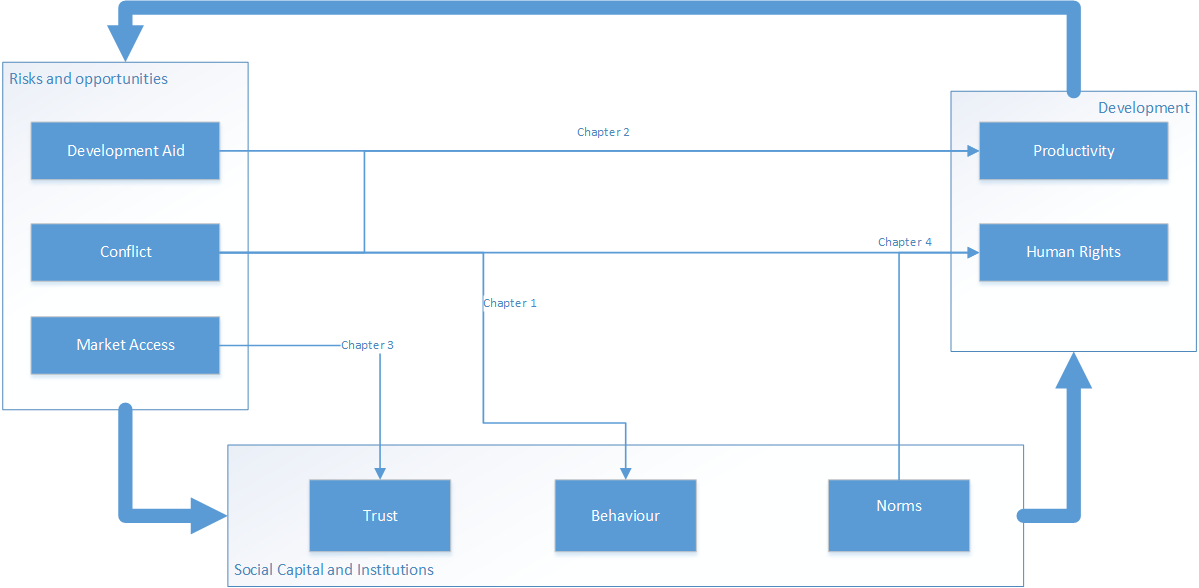
\includegraphics[width=0.8\linewidth]{"\git/thesis/analysis/introduction/figures/conceptual_framework.png"}
  \caption{Conceptual Framework}
  \label{intro:fig:framework}
\end{figure}


\section{Risks and Oportunities}
I focus on three sources of risks and opportunities for development. 

The first is violent conflict. The 2011 World Development Report was titled Conflict, Security, and Development, underscoring the importance of violent conflict in shaping development outcomes \cite{WorldBank2011}. \citet{Collier2003} has labelled conflict ``Development in Reverse''. Aside from the human rights violations that are inherent to violent conflict, other consequuences include: decreased economic activity \citep{Collier1999} deforestation \cite[e.g.][]{Connectiona}, long-term incidence of domestic violence \citep[e.g.][]{LaMattina2017; Muller2019}, (mental) health problems \cite[e.g.][]{Smith2002; Iqbal2006a;Akresh2011}, food insecurity \cite[e.g.][]{Lecoutere2005; Verwimp2012}... However, some more positive effects have been described, such as increased collective action \citep{Bellows2009b}, political participation \citep{Blattman2009a} and increased pro-social behaviour \citep{Voors2012a}.

Next, I consider an opportunity for development: markets. Markets provide opportunities for exchange and specialization, which can boost economic development. 

Thirdly,  development aid. The lack of state capacity makes it hard to fulfil citizen's needs for healthcare, education, and services, leading to international donors to attempt and alleviate the resulting humanitarian crises.

\section{Social Capital and Institutions}
The impact that these risks and opportunities can have differ widely over countries. Some countries have been better able to exploit the advantages markets offer than others; some conflicts have larger consequences than others. The key factor that sets apart countries that are succesful in avoiding risk and copitalizing on opportunities is, is the institutional environment \citep{Rodrik2004,Acemoglu2000}. This term is used to describe the rules and norms that shape (economic) life. It covers crucial things such as protection of property rights and equal treatment by the law \citep{Acemoglu2005}. Such good institutions  foster development by incentivizing innovation. However, the relationship between institutions and development does not run in one direction. While institutions cause growth \citep{Acemoglu2000}, the economic growth that accompanies development also allows for better institutions. It is possible that countries could enter a virtuous cycle, where improved institutional quality enhances growth, which improves institutional quality \citep{Voors2011}.

%
Social capital is closely related to institutions. \todo{what is social capital?} Especially in poorer countries, social capital plays an important role in facilitating economic activity \citep{Knack1997}. In such countries, social capital may be a substitute for formal institutions by providing insurance and securing property rights. To a large extent, such social capital is underpinned by pro-social behaviour. \todo{really?}

%However, institutions can also increase cooperative behaviour \citep{Bo2008,Henrich2010}. 
This implies that countries with a high level of social capital or good institutions can enter a virtuous cycle of institutions producing growth and social capital; and social capital and growth producing quality institutions. The question on how to enable such a virtuous cycles for fragile states is too large for any one thesis. This thesis aims to provide empirical, micro-level level evidence on how social capital and behaviour mediate development in fragile states. Figure \ref{intro:fig:framework} outlines these concepts. Each chapter in this thesis then explores one subset of the possible relationships within the framework.



\section{Development}
As for development, I focus on agricultural productivity and human rights. I focus on agricultural production, as the poorest of the world often depend on subsistence agriculture. Furthermore, agricultural productivity is seen as a necessary precondition for further, economy-wide, productivity improvements. \todo{why?} 

However, a focus on productivity is too narrow to fully capture the problems that life in fragile states presents in terms of development. Productivity gains mean little in the face of widespread human rights violations. Human dignity is a crucial part of development.


\section{Research Questions}
The questions this thesis aims to answer are:
\begin{enumerate}
	\item What is the relationship between conflict and competitive behaviour? (Chapter \ref{chap:slfootball});
	\item What is the effect of input subsidies on novel technology adoption? (Chapter \ref{chap:n2a_impact});
	\item What is the effect of market access on trusting behaviour (Chapter \ref{chap:cameroontrust}); and,
	\item What are the drivers of sexual and gender-based violence in Eastern Congo (Chapter \ref{chap:congogbv}).
\end{enumerate}

\section{Contribution}
The primary contribution of this thesis lies in the collection of large-scale datasets in fragile states. This fits within a broader trend where the amount of data collected in such states has increased over the past decades. Two factors contribute to this increase. On the supply side, cost of data collection is dropping. Information technology allows for cheaper collection and processing of data, and for more effective monitoring of field staff. On the demand side, is a drive to more rigorously evaluate the impact development aid. This necessitates the collection of detailed household-level data to compare project beneficiaries with non-beneficiaries. The primary funding for this PhD-thesis comes from such an evaluation: the MFS II evaluations, commissioned by the Dutch ministry of foreign affairs.

Despite this increase in data collection efforts, citizens of Fragile States remain under-represented in studies on behaviour. Chapter \ref{chap:slfootball} contributes by studying the effects of conflict on youth in Sierra Leone. Chapter \ref{chap:cameroontrust} contributes to this by collecting large-scale data on behaviour of an understudied group: Africans from rural areas, with poor access to markets. Chapter 4 studies the dynamics of sexual violence in Congo. Despite the prominence the topic has had in public discourse on Congo, and despite its severity, little data exists on these dynamics. This is partly due the difficulties and costs inherent in operating in unstable countries.

All data sets used for analyses, and all protocols and analysis scripts are released to the public domain.


\section{Outline}


%bibliography, this is needed for bibtex
\clearpage 
\bibliographystyle{chicago}
%path to .bib file (e.g. automatically exported by mendeley) DO NOT include the file extension!
\bibliography{\dropbox/Literatuur/Mendeley/Bibtex/Thesis-Introduction}